\chapter{Introduction to Set Theory}
\label{chp:set_theory}
Set theory is a fundamental branch of mathematical logic that underpins much of mathematics, including probability theory. At its core, set theory concerns the concept of a set -- a collection of distinct objects or elements. This introduction explores the essential properties and operations of sets to lay the groundwork for the axiomatic development of probability theory and statistics.


\begin{definition}[Membership]
	In set theory, the membership relation between an object $o$ and a set $A$ is fundamental. $o \in A$ denotes that $o$ is an element or member of $A$.
\end{definition}

\begin{definition}[Set]
	A set\index{Set} is a collection of distinct objects, considered as an object in its own right. Sets are typically denoted using curly braces $\{\}$ and can be described in two primary ways:
	\begin{enumerate}
		\item By listing its elements separated by commas, e.g., $A = \{a_1, a_2, a_3\}$.
		\item By specifying a characterizing property of its elements, e.g., \newline $A = \{x \mid x \text{ is a natural number}\}$.
	\end{enumerate}
	Sets can also be illustrated graphically, as shown in \figref{fig:generic_set}.
	\begin{figure}[H]
		\centering
		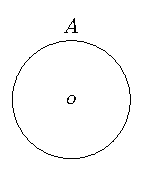
\includegraphics[width = 0.35\textwidth]{figures/generic_set.pdf}
		\caption{The graphical representation of a generic set $A$ with generic elements $o$.}
		\label{fig:generic_set}
	\end{figure}
\end{definition}

\begin{definition}[Subset]
	A set $A$ is called a subset\index{Subset} of a set $B$, denoted $A \subseteq B$, if every element of $A$ is also an element of $B$. Formally, $A\subseteq B$ if $\forall x \in A, x \in B$. By this definition, a set is always a subset of itself.
	\begin{figure}[H]
		\centering
		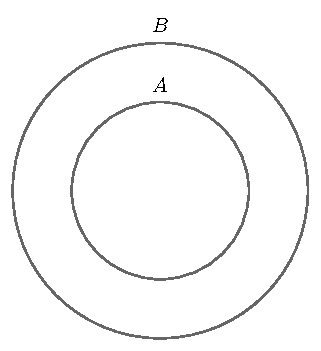
\includegraphics[width = 0.5\textwidth]{figures/set_subset.pdf}
		\caption{The graphical representation of $A\subseteq B$.}
		\label{fig:set_subset}
	\end{figure}
\end{definition}

\begin{definition}[Proper Subset]
	A set $A$ is called a proper subset of a set $B$, denoted $A \subset B$, if $A \subseteq B$ and $A \neq B$. This means that $A$ is a subset of $B$ but $A$ is not equal to $B$; there is at least one element in $B$ that is not in $A$.
\end{definition}

\begin{example}
	Suppose $A = \{\twemoji{banana}, \twemoji{apple}, \twemoji{eggplant}\}$, then $\{\twemoji{banana}, \twemoji{apple}\}$ and $\{\twemoji{apple}\}$ are proper subsets of $A$, meaning $\{\twemoji{banana}, \twemoji{apple}\},\{\twemoji{apple}\}\subset  A$. $\{\twemoji{banana}, \twemoji{carrot}\}$, on the other hand, is not a subset of $A$, meaning $\{\twemoji{banana}, \twemoji{carrot}\}\not\subset  A$.
\end{example}
\begin{example}
	$\twemoji{banana}$, $\twemoji{apple}$, and $\twemoji{eggplant}$ are members (elements) of the set $\{\twemoji{banana}, \twemoji{apple}, \twemoji{eggplant}\}$, but are not subsets of it; and in turn, the subsets, such as $\{\twemoji{banana}\}$, are not members of the set $\{\twemoji{banana}, \twemoji{apple}, \twemoji{eggplant}\}$.
\end{example}

\begin{definition}[Empty Set]
	The empty set\index{Empty set}, denoted by $\emptyset$ or $\{\}$, is the set that contains no elements.
\end{definition}

\begin{definition}[Universal Set]
	The universal set\index{Universal set}, denoted by $\Omega$, is the set that contains all the objects or elements under consideration in a particular discussion or problem. It is the largest set in the context of a given study.
\end{definition}

\begin{definition}[Closure]
	A set $A$ is said to be \textit{closed} under a certain operation if, for every pair of elements $x$ and $y$ in $A$, the result of applying the operation to $x$ and $y$ is also in $A$.
\end{definition}

\begin{definition}[Union]
	The union of sets $A$ and $B$, denoted by $A \cup B$, is defined as the set containing all elements that are in $A$ or $B$ (or both). \figref{fig:set_union} provide a graphical representation of $A \cup B$.
	\begin{figure}[h]
		\centering
		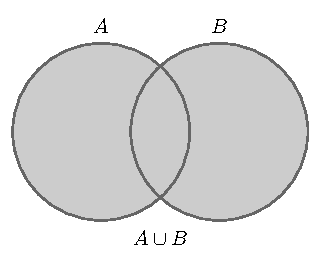
\includegraphics[width = 0.6\textwidth]{figures/set_union.pdf}
		\caption{The figure show the union of sets $A$ and $B$. Each circle represent the sets and the colored region represent the result of the result of the binary operation.}
		\label{fig:set_union}
	\end{figure}
\end{definition}

\begin{definition}[Intersection]
	The intersection of sets $A$ and $B$, denoted by $A \cap B$, is defined as the set containing all elements that are common to both $A$ and $B$. \figref{fig:set_intersection} provide a graphical representation of $A \cap B$.
	\begin{figure}[H]
		\centering
		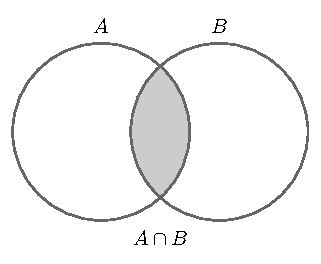
\includegraphics[width = 0.6\textwidth]{figures/set_intersection.pdf}
		\caption{The figure show the intersection of sets $A$ and $B$. Each circle represent the sets and the colored region represent the result of the result of the binary operation.}
		\label{fig:set_intersection}
	\end{figure}
\end{definition}

\begin{definition}[Disjoint]
	Two sets $A$ and $B$ are said to be disjoint if their intersection is the empty set, i.e., $A \cap B = \emptyset$. \figref{fig:set_disjoint} provide a graphical representation of $A \cap B=\emptyset$.
	\begin{figure}[H]
		\centering
		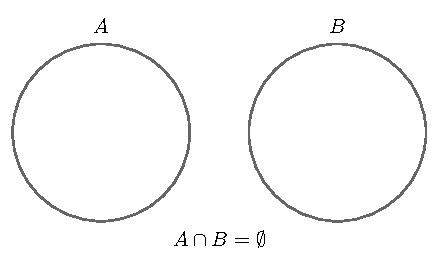
\includegraphics[width = 0.8\textwidth]{figures/set_disjoint.pdf}
		\caption{The figure show the case where the intersection of sets $A$ and $B$ is the empty set. Each circle represent the sets and the colored region represent the result of the result of the binary operation.}
		\label{fig:set_disjoint}
	\end{figure}
\end{definition}


\begin{definition}[Complementation]
	The complement of set $A$, denoted by $A^c$, is defined as the set containing all elements in the universal set $\Omega$ that are not in $A$. \figref{fig:set_complementation} provide a graphical representation of $(A \cap B)^c$.
	\begin{figure}[H]
		\centering
		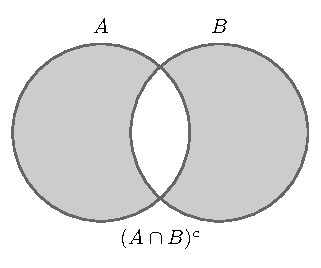
\includegraphics[width = 0.6\textwidth]{figures/set_complementary.pdf}
		\caption{The figure show the complementary of the intersection of sets $A$ and $B$. Each circle represent the sets and the colored region represent the result of the result of the binary operation.}
		\label{fig:set_complementation}
	\end{figure}
\end{definition}

\begin{definition}[Difference]
	The difference between set $A$ and $B$, denoted by $A \setminus B = A\cap B^c$, is defined as the set containing all elements in $A$ that are not in $B$. \figref{fig:set_minus} provide a graphical representation of $A\setminus B$ and $B\setminus A$.
	\begin{figure}[H]
		\centering
		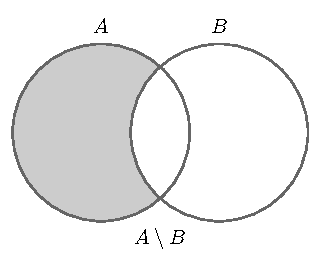
\includegraphics[width = 0.6\textwidth]{figures/set_minus.pdf}
		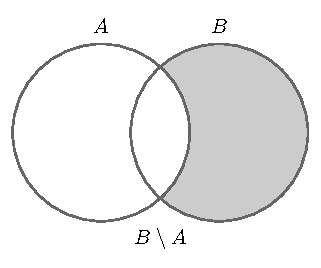
\includegraphics[width = 0.6\textwidth]{figures/set_minus2.pdf}
		\caption{(top) show $A$ minus $B$ and (bottom) show $B$ minus $A$. Each circle represent the sets and the colored region represent the result of the result of the binary operation.}
		\label{fig:set_minus}
	\end{figure}
\end{definition}

\begin{definition}[Power Set]
	The power set\index{Power set} of a set $A$, denoted by $2^A$, is defined as the set containing all possible subsets of $A$, including $A$ itself and the empty set.
\end{definition}

\begin{example}
	Suppose $A = \{a_1,a_2,a_3\}$, then
	\begin{equation}
		\begin{split}
			2^A = \{&\emptyset, \{a_1\}, \{a_2\}, \{a_3\}, \{a_1, a_2\},\\
			& \{a_1, a_3\}, \{a_2, a_3\}, \{a_1, a_2, a_3\}\}.
		\end{split}
	\end{equation}
\end{example}

\begin{definition}[Symmetric Difference]
	The symmetric difference of sets $A$ and $B$, denoted by $A \Delta B$, is defined as the set containing all elements that are in either $A$ or $B$ but not in both, meaning $A \Delta B = (A \cap B)^c$. \figref{fig:set_complementation} show the symmetric difference between sets $A$ and $B$.
\end{definition}

\begin{definition}[Finite and Infinite Unions]
	For a collection $\{A_i\}$, the union is denoted by $\bigcup_{i} A_i$ and is defined as the set containing all elements that are in at least one of the sets $A_i$.
\end{definition}

\begin{definition}[Partition]
	A collection of non-empty subsets $\{A_i\}$ of a set $A$ is called a partition of $A$ if the following conditions are satisfied:
	\begin{enumerate}
		\item The subsets $A$ are pairwise disjoint, i.e., $A_i \cap A_j = \emptyset$ for all \(i \neq j\).
		\item The union of all subsets \(A_i\) is equal to the set \(A\), i.e., \(\bigcup_{i \in I} A_i = A\).
	\end{enumerate}
	
	A graphical representation of the set $A=\{A_1,A_2,A_3\}$, where $A_j$ are partitions, is shown in \figref{fig:set_partition}.
	\begin{figure}[h]
		\centering
		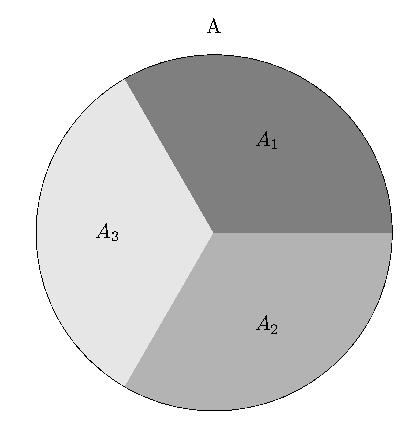
\includegraphics[width = 0.6\textwidth]{figures/set_partition.pdf}
		\caption{The figure show $A=\{A_1,A_2,A_3\}$ where $A_j$ are partitions.}
		\label{fig:set_partition}
	\end{figure}
\end{definition}


\begin{definition}[Finite and Infinite Intersections]
	For a collection $\{A_i\}$, the intersection is denoted by $\bigcap_{i} A_i$ and is defined as the set containing all elements that are common to all sets $A_i$.
\end{definition}

\begin{definition}[Cartesian Product]
	The Cartesian product of sets $A$ and $B$, denoted by $A \times B$, is defined as the set containing all ordered pairs $(a, b)$, where $a$ is in $A$ and $b$ is in $B$.
\end{definition}

\begin{example}
	Suppose $A= \{a_1,a_2\}$ and $B=\{b_1,b_2,b_3\}$, then
	\begin{equation}
		\begin{split}
			A\times B = \{&(a_1,b_1),(a_1,b_2),(a_1,b_3),\\
			&(a_2,b_1),(a_2,b_2),(a_2,b_3)\}
		\end{split}
	\end{equation}
\end{example}

	
